%%%%%%%%%%%%%%%%%%%%%%%%%%%%%%%%%%%%%%%%%%%%%%%%%%%%%%%%%%%%%%%%%%%%%%
%%  
%%  UOIT-THESIS.TEX
%%
%% This program can be redistributed and/or modified under the terms
%% of the LaTeX Project Public License Distributed from CTAN archives
%% in directory CTAN:/macros/latex/base/lppl.txt.
%%
%% Copyright (c) 2010 by Faisal Qureshi
%% Last Update: 2010 December 20
%%
%%%%%%%%%%%%%%%%%%%%%%%%%%%%%%%%%%%%%%%%%%%%%%%%%%%%%%%%%%%%%%%%%%%%%%
%%
%% Thanks to Francois Pitt for letting me use his ut-thesis.tex and
%% ut-thesis.cls files for my purposes.
%%
%% Based upon ut-thesis.tex
%%
%% Copyright (c) 1999 by Francois Pitt
%% Last Update: 1999 May 13
%%  
%%%%%%%%%%%%%%%%%%%%%%%%%%%%%%%%%%%%%%%%%%%%%%%%%%%%%%%%%%%%%%%%%%%%%%
%%  
%%  This file is distributed in the hope that it will be useful but
%%  without any warranty (without even the implied warranty of
%%  fitness for a particular purpose).  For a description of this
%%  file's purpose, and instructions on its use, see below.
%%  
%%  Feel free to copy and redistribute this file, as long as this
%%  copyright notice remains intact and this file is distributed
%%  along with the companion file `uoit-thesis.cls'.
%%  
%%  (Thanks to Robert Bernecky for his suggestions on improving the
%%  usefulness and readability of this file.)
%%  
%%  Send all bugs, questions, comments, suggestions, etc. to the
%%  author, at <faisal.qureshi@uoit.ca>.
%%  
%%%%%%%%%%%%%%%%%%%%%%%%%%%%%%%%%%%%%%%%%%%%%%%%%%%%%%%%%%%%%%%%%%%%%%
%%  
%%  To be used in conjunction with class file `uoit-thesis.cls', whose
%%  features it illustrates.
%%  
%%  To comment out parts of a file, use the macro \ignore{...}
%%  around the entire block of text you want to ignore.
%%  
%%  To explicitly set the pagestyle of any inserted blank page when
%%  \cleardoublepage occurs, use one of \clearemptydoublepage or
%%  \clearplaindoublepage instead.
%%  
%%  For single-spaced quotes or quotations, use the `longquote' and
%%  `longquotation' environments.  For single-spaced, 1 1/2-spaced,
%%  or double-spaced paragraphs, use one of the environments
%%  `singlespaced', `oneandahalfspaced', or `doublespaced'.  More
%%  generally, for paragraphs with a line spacing of `n', use
%%  `\begin{newspacing}{n}...\end{newspacing}'.
%%  
%%  All other environments, commands, and options provided by the
%%  `ut-thesis' class will be described below, at the point where
%%  they should appear in the document.
%%  
%%  See the companion file `uoit-thesis.cls' for more details.
%%  
%%%%%%%%%%%%%%%%%%%%%%%%%%%%%%%%%%%%%%%%%%%%%%%%%%%%%%%%%%%%%%%%%%%%%%


%%%%%%%%%%%%         PREAMBLE         %%%%%%%%%%%%

%% Default settings format a final copy (12pt font, single-sided,
%% double-spaced, normal margins, single-spaced notes).  For a rough
%% copy (10pt font, double-sided, double-spaced, normal margins, with
%% the word "DRAFT" printed at each corner of every page), use the
%% `draft' option.  The default line spacing can be changed with one
%% of the following options: `singlespaced', `oneandahalfspaced', or
%% `doublespaced'.  The notes are always single-spaced by default, but
%% can be made to have the same spacing as the rest of the document by
%% using the option `spacednotes'.  The size of the margins can be
%% changed with one of the following options: `narrowmargins' (1 1/4"
%% left, 3/4" others), `normalmargins' (1 1/4" left, 1" others),
%% `widemargins' (1 1/4" all), `extrawidemargins' (1 1/2" all).  Any
%% other standard option for the `report' document class can be used
%% to override the default or draft settings.

%% For "undergraduate theses", uncomment the following line and 
%% add any other options that you may require 
\documentclass{uoit-thesis}

%% For "graduate thesis" use the 'grad' option, uncomment the
%% following line and any other options that you may require
%% \documentclass[grad]{uoit-thesis}

%% ***   Add \usepackage declarations here.   ***

\usepackage[
  % Some remarks:
  % * drivers like 'pdftex' that can be detected automatically
  %   are not necessary
  % * breaklinks is rather an internal option.
  %   If a driver does not support it, then forcing the option
  %   let the text break across lines, but also the link
  %   areas are "broken". If the driver supports the option,
  %   then the option is enabled anyway.
  % * Information entries should be set outside,
  %   because LaTeX expands the package options,
  %   hyperref does not like them, if they are
  %   prematurely expanded.
  % * Hyperref has a new option for hiding links: hidelinks
  % hidelinks,
  colorlinks,
  citecolor=darkgreen,
  filecolor=black,
  linkcolor=darkblue,
  urlcolor=blue,
  %%letterpaper,
  linktoc=all,
  pagebackref,
  bookmarksopen,
  bookmarksnumbered,
]{hyperref}
\hypersetup{
  pdfauthor={Pat Goebel},
  % ...
}
% Adding package bookmark improves bookmarks handling.
% More features and faster updated bookmarks.
\usepackage{bookmark}

\usepackage{tikz,pgfplots}

\usepackage{caption}

\usetikzlibrary{intersections}
\pgfplotsset{compat=1.8}

% \usepackage{pst-all}z
% \usepackage{pstricks-add}
% \usepackage{lmodern}
% \usepackage{graphicx}
% \usepackage[miktex]{gnuplottex}
% \usepackage{epstopdf}

\usepackage{float}

\usepackage{lmodern}
\usepackage[T1]{fontenc}

% \usepackage{inconsolata}
% \renewcommand*\familydefault{\ttdefault} %% Only if the base font of the document is to be typewriter style
% \usepackage[T1]{fontenc}

%% The line spacing of the document should be specified using one of
%% the document options given above, but if you need a line spacing
%% that is not provided by the options, you can override the default
%% line spacing for the entire document with the command
%%   `\linespacing{...}'.
%% Note that in order to get the correct appearance, the argument to
%% `\linespacing' must be equal to 1/3 + 2/3 times the desired line
%% spacing (for example, single-spaced = \linespacing{1},
%%                        1 1/2-spaced = \linespacing{1.33}, and
%%                       double-spaced = \linespacing{1.66}).

%% ***   Uncomment and fill in a value, if needed.    ***
%% ***   REMEMBER: You should NOT need to use this.  Use one of   ***
%% ***   the document class options mentionned above instead.     ***
%\linespacing{}




%%%%%%%%%%%%%%%%%%%%%%%%%%%%%%%%%%%%%%%%%%%%%%%%%%%%%%%%%%%%%%%%%%%%%%
%%                                                                  %%
%%                  ***   I M P O R T A N T   ***                   %%
%%                                                                  %%
%%  Fill in the following fields with the required information:     %%
%%   - \degree{...}       name of the degree obtained               %%
%%   - \faculty{...}      name of the faculty                       %%
%%   - \department{...}   name of the program                       %%
%%   - \gradyear{...}     year of graduation                        %%
%%   - \author{...}       name of the author                        %%
%%   - \title{...}        title of the thesis                       %%
%%%%%%%%%%%%%%%%%%%%%%%%%%%%%%%%%%%%%%%%%%%%%%%%%%%%%%%%%%%%%%%%%%%%%%

%% ***   Change this example to appropriate values.   ***
\degree{Bachelor of Science}
\faculty{Science}
\department{Computing Science}
\gradyear{2014}
\supervisor{Dr ~F. ~Z. Qureshi}
\author{Pat C. Goebel}
\title{Fast image matching using ORB and Multi-Index Hashing}

%% ***   NOTE   ***
%% Put here all other formatting commands that belong in the preamble.


%% For example, to list only down to subsections in table of contents
%% (-1=part, 0=chapter, 1=section, 2=subsection, 3=subsubsection,
%%  4=paragraph, 5=subparagraph, 6=subsubparagraph).
%
\setcounter{tocdepth}{2}


%%%%%%%%%%%%      MAIN  DOCUMENT      %%%%%%%%%%%%

\begin{document}

% \newcommand*{\myfont}{\fontfamily{fi4}\selectfont}
\newcommand{\figfont}{\scriptsize \sffamily}


\definecolor{bfeat1}{RGB}{255, 0, 0}
\definecolor{bfeat2}{RGB}{0, 0, 255}
\definecolor{bfeat3}{RGB}{0, 255, 0}
\definecolor{bfeat4}{RGB}{191, 128, 64}
\definecolor{bfeat5}{RGB}{0, 128, 128}
\definecolor{bfeat6}{RGB}{255, 128, 0}
\definecolor{bfeat7}{RGB}{128, 0, 128}
\definecolor{bfeat8}{RGB}{0, 0, 0}

\definecolor{darkblue}{RGB}{0, 0, 143}
\definecolor{darkgreen}{RGB}{0, 80, 0}

\pgfplotscreateplotcyclelist{colorbfeat}{
{bfeat8},
{bfeat1},
{bfeat2},
{bfeat3},
{bfeat4},
{bfeat5},
{bfeat6},
{bfeat7},
}

\newcommand{\testplot}{
\begin{tikzpicture}
\begin{axis}[domain=-10:10, samples=50, smooth, no markers, enlargelimits=false]
\addplot gnuplot {sin(x)}; \addlegendentry{$\sin(x)$}
\addplot gnuplot {cos(x)}; \addlegendentry{$\cos(x)$}
\end{axis}
\end{tikzpicture}
}


%% arguments are file, title, number of descriptors queried
\newcommand{\plottestIII}[3]{
\begin{tikzpicture}
\begin{axis}[
    height=5cm,
    width=10cm,
    title={#2},
%     restrict x to domain=0:1500,
    xmax=1300,
    xmin=0,
    xtick={1,250,500,750,1000},
    enlarge y limits=0,
    enlarge x limits=0.025,
    cycle list name=colorbfeat,
    no markers,
    legend style={legend pos=north east,font=\tiny},
    scaled ticks=false,
    tick label style={/pgf/number format/fixed},
    ylabel near ticks,
    xlabel near ticks,
    ylabel={Query time in $s$},
    xlabel={k-NN},
]
    \pgfplotstableread{#1}{\table}
    \pgfplotstablegetcolsof{#1}
    \pgfmathtruncatemacro\numberofcols{\pgfplotsretval-1}
    \pgfplotsinvokeforeach{1,...,\numberofcols}{
        \pgfplotstablegetcolumnnamebyindex{##1}\of{\table}\to{\colname}
        \addplot+[thick] table [y index=##1, y expr=\thisrow{\colname}/(1000000000)/(#3)] {#1};
        \addlegendentryexpanded{\colname}
    }
\end{axis}
\end{tikzpicture}
}

\newcommand{\plottestIV}[3]{
\begin{tikzpicture}
\begin{axis}[
    height=4cm,
    width=0.29\textwidth,
%     axis x line=bottom,
%     axis y line=left,
%     axis on top,
%     grid=minor,
%     minor ytick={0.5},
%     ytick={0.1,0.2,0.3,0.4,0.5,0.6},
    title={#2},
    ybar interval,
%     ybar,
    ymin=0,
%     restrict x to domain=0:255,
    x tick label as interval=false,
    xtick={},
%     xtick={0,64,128,192,255},
    xmajorgrids=false,
    ymajorgrids=false,
    bar width=0.8,
%     x=1,
    xmax=85,
    xmin=15,
    scaled ticks=false,
    tick label style={/pgf/number format/fixed},
    enlarge x limits=0.01,
    ylabel near ticks,
    xlabel near ticks,
    ylabel={Fraction of queries},
    xlabel={Hamming radii needed for #3-NN},
]
\addplot[fill=darkblue, draw opacity=0] table {#1};
\end{axis}
\end{tikzpicture}
}

% \newcommand{\plottestV}[2]{
% \begin{tikzpicture}
% \begin{axis}[
%     height=4cm,
%     axis x line=bottom,
%     axis y line=left,
%     axis on top,
%     grid=minor,
%     minor ytick={0.5},
%     ytick={0.1,0.2,0.3,0.4,0.5,0.6},
%     title={#2},
%     ybar interval,
%     ymin=0,
%     restrict x to domain=0:255,
%     x tick label as interval=false,
% %     xtick={},
%     xtick={0,64,128,192,255},
%     xmajorgrids=false,
%     ymajorgrids=false,
%     x=1,
%     enlarge x limits=0.01,
%     ylabel near ticks,
%     xlabel near ticks,
%     ylabel={Proportion set to 1},
%     xlabel={bit \#},
% ]
% \addplot[fill=blue, draw opacity=0] table {#1};
% \end{axis}
% \end{tikzpicture}
% }


\newcommand{\plottestV}[4]{
\begin{tikzpicture}
\begin{axis}[
    height=4cm,
    axis x line=bottom,
    axis y line=left,
    axis on top,
    grid=minor,
    minor ytick={0.5},
    ytick={0.1,0.2,0.3,0.4,0.5,0.6},
    title={#2},
    ybar interval,
    ymin=0,
    restrict x to domain=0:255,
    x tick label as interval=false,
%     xtick={},
    xtick={0,64,128,192,255},
    xmajorgrids=false,
    ymajorgrids=false,
    xmin=0,
    xmax=255,
    x=1,
    enlarge x limits=0.01,
    ylabel near ticks,
    xlabel near ticks,
    ylabel={Proportion set to 1},
    xlabel={bit \#},
]
\addplot[fill=green, draw opacity=0, restrict y to domain=#3:#4] table {#1};
\addplot[fill=red, draw opacity=0, ignore points in y range=#3:#4] table {#1};
\end{axis}
\end{tikzpicture}
}

% argument is number of samples
\newcommand{\plotchisqr}{
\addplot[name path global=GraphCurve, mark=none, domain=-2.5:2.5, thick] ({x},{x*x});
}

%% ***   NOTE   ***
%% You should put all of your `\newcommand', `\newenvironment', and
%% `\newtheorem's (in other words, all the global definitions that
%% you will need throughout your thesis) in a separate file and use
%% "\input{filename}" to input it here.


%% This sets the page style and numbering for preliminary sections.
\begin{preliminary}

%% This generates the title page from the information given above.
\maketitle

%% There should be NOTHING between the title page and abstract.

%% This generates the abstract page, with the line spacing adjusted
%% according to SGS guidelines.
\begin{abstract}
We have combined the Multi-Index Hashing technique with large binary descriptors to provide fast, accurate image matching in large datasets. We have found that 256 bit rotated BRIEF descriptors generated with the oriented FAST feature detector can be matched in sub-linear time. We have shown this technique to be effective for databases of up to 10 million codes generated from 25,000 images. This research shows that accurate matching of images is possible for large image datasets while maintaining speed and space efficiency by coupling natively generated binary image descriptors with the Multi-Index Hashing technique.
%% ***   Put your Abstract here.   ***
%% (At most 150 words for M.Sc. or 350 words for Ph.D.)
\end{abstract}

%% Anything placed between the abstract and table of contents will
%% appear on a separate page since the abstract ends with \newpage
%% and the table of contents starts with \clearpage.

%% This generates a "dedication" section, if needed.
%% (uncomment to have it appear in the document)
%\begin{dedication}
%% ***   Put your Dedication here.   ***
%\end{dedication}

%% The `dedication' and `acknowledgements' sections do not create new
%% pages so if you want the two sections to appear on separate pages,
%% you should put an explicit \newpage between them.

%% This generates an "acknowledgements" section, if needed.
%% (uncomment to have it appear in the document)
%\begin{acknowledgements}
%% ***   Put your Acknowledgements here.   ***
%\end{acknowledgements}

%% This generates the Table of Contents (on a separate page).
\begingroup
\hypersetup{linkcolor=black}
\tableofcontents
\endgroup

%% This generates the List of Tables (on a separate page), if needed.
%% (uncomment to have it appear in the document)
%\listoftables

%% This generates the List of Figures (on a separate page), if needed.
%% (uncomment to have it appear in the document)
%\listoffigures

%% End of the preliminary sections: reset page style and numbering.
\end{preliminary}

%%%%%%%%%%%%%%%%%%%%%%%%%%%%%%%%%%%%%%%%%%%%%%%%%%%%%%%%%%%%%%%%%%%%%%
%%  Put your Chapters here; the easiest way to do this is to keep   %%
%%  each chapter in a separate file and `\include' all the files    %%
%%  right here.  Note that each chapter file should start with the  %%
%%  line "\chapter{ChapterName}".  Note that using `\include'       %%
%%  instead of `\input' makes each chapter start on a new page.     %%
%%%%%%%%%%%%%%%%%%%%%%%%%%%%%%%%%%%%%%%%%%%%%%%%%%%%%%%%%%%%%%%%%%%%%%

%% ***   Include chapter files here.   ***
\chapter{Introduction}
\section{Thesis Statement}
We aim to explore the effectiveness of the Multi-Index Hashing technique~\cite{norouzi2012fast} for the fast matching of large, binary, image descriptors in large databases for the purpose of fast, accurate image matching.

\section{Background: Problem and Related Work}
Image matching is an active area of research with wide ranging applications, but achieving good performance with respect to speed, space and accuracy is still a challenge. There has been growing interest in mapping image data onto compact binary codes for fast nearest neighbours search. Binary codes are storage efficient and comparisons require just a small number of machine instructions, such that millions of binary codes can be compared to another in less than a second. Binary codes can also be used as direct indices into hash tables which can provide constant time lookups. In spite of the efficiency and speed of using binary codes to represent image data, most image feature description is expressed as vectors of floating point numbers which must be compared using a measure of Euclidean distance. While there has been work on mapping these real valued descriptors to binary codes ~\cite{torralba2008small,norouzi2011minimal} the issue remains that these schemes provide an imperfect mapping from real valued vectors to binary codes, and that to achieve a strong correlation between the Euclidean distance for the real valued codes and the Hamming distance for the binary codes, large binary code lengths must be used. While matching long binary codes is still quite fast using linear scanning, they have posed a problem in that up until recently it was inefficient to quickly match binary codes longer than 30 bits ~\cite{torralba2008small} using the binary codes as indices into hash tables. With the introduction of the MIH technique it is possible to exactly match codes longer than \textasciitilde30 bits faster than linear scanning.

\subsection{Motivation}
The motivation behind this work is the ability for the MIH technique to enable the use of high performance binary descriptors such as Rotated BRIEF. Binary descriptors do have the advantage of being easy to compare because Hamming distance is easily computed and is efficient on computer systems, but current limitations significantly decrease the efficiency of using longer binary codes which can have better matching properties than popular Euclidean distance based descriptors such as SIFT and SURF ~\cite{rublee2011orb}. With the MIH method of calculating Hamming space nearest neighbours we gain performance in matching long binary codes. This performance gain is helpful for the hashing techniques on real valued descriptors, but also enables the use of natively generated binary descriptors which do not suffer from the degradation of matching rates (See Figure ~\ref{fig:hashmatching}) due to hashing from Euclidean to binary descriptors, are faster to generate, and allow better matching properties.

\subsection{Multi-Index Hashing}
The Multi-Index Hashing technique introduces a fast method of searching for exact k-nearest neighbours in hamming space which is also space efficient~\cite{norouzi2012fast} . Previous solutions were using binary codes as direct indices into hash tables but this approach was not used for codes longer than 32 bits because the memory requirements are prohibitive~\cite{torralba2008small}. While the direct hashing is fast for shorter binary codes, it is desirable to use longer codes as short codes do not preserve similarity as well.

In the research introducing the MIH technique, an emphasis is placed on the mathematical properties of the proposed data structure, but empirical analysis of the structure was carried out using 64 and 128 bit codes, generated using Locality Sensitive Hashing and Minimal Loss Hashing from SIFT and GIST descriptor datasets. Analysis of the performance properties of 256 bit codes was not included in the research so we sought to analyze the performance of MIH using 256 bit codes.
\chapter{Methods}

\section{Definitions}
\begin{description}
 \item[ORB] Oriented FAST and rotated BRIEF
 \item[LSH] Locality-sensitive hashing
 \item[MLH] Minimal Loss Hashing
 \item[MIH] Multi-Index Hashing
\end{description}

\section{General System Overview}
This thesis integrates an Oriented FAST and Rotated BRIEF (ORB) feature detection and description module with a Multi-Index Hashing library. Our design utilized the ORB feature detector and descriptor extractor to generate 256 bit feature descriptor codes. These codes were then used to populate the multi-index hashing (MIH) data structure. The populated MIH structure was then queried using the provided interface.

To generate our list of binary codes we iterate through images in a directory and for each image we preprocess it by converting it to grayscale and applying a gaussian blur with radius 7 to eliminate noise. After the image has been preprocessed it is passed to ORB to generate features, then binary descriptors. For each image these descriptors are appended to a list of descriptors. When all the images have been iterated through we then can use the full list of descriptors to pass to an instance of the MIH datastructure to populate it.

A facility was created to serialize and deserialize the generated descriptors as to avoid generating the descriptors for every test.

\section{ORB Module}
The ORB module is part of the OpenCV library~\cite{rublee2011orb}. ORB takes as an input one image file and outputs a list of binary descriptors extracted from that image. In this paper, binary descriptors are defined as binary codes which represent the salient features of the image they are produced from. Any image file that OpenCV can read and process can be passed to ORB. The ORB processes these images into binary descriptors by using two sub-components: The Oriented Fast Feature Detector (FD) component, followed by the Rotated BRIEF Descriptor Extractor (DE).

The FD uses corner detection with an intensity centroid orientation measure as well as a scale pyramid which are passed through a Harris corner filter to eliminate edge matches, producing corner descriptors that have scale and orientation information~\cite{rublee2011orb}. These features are then passed onto the DE. The DE takes the image, a keypoint and the feature information and computes a binary code which represents that feature~\cite{rublee2011orb}.

The authors of the ORB module in OpenCV chose a descriptor length of 256 bits for the output of the DE and this defined the size of binary codes used for our experiments.

\section{MIH library}
The MIH technique works by splitting every code used to populate the structure into $m$ disjoint substrings and using these substrings as indices into $m$ different hash tables. This allows us to search many fewer buckets in the hash tables as we know that, given a query radius of $r$, any code within this radius from the query will have at least one substring which differs by at most $\lfloor \frac{r}{m} \rfloor$ bits. This provides sub-linear query times for large databases of large codes.
 
The MIH code was modified to remove dependencies on MATLAB and was compiled as a library to be linked to by our code. 256 bit binary codes were used to populate the MIH structure and performance tests were carried out by querying the MIH structure, varying the number of neighbours searched for and by varying the substring length used by MIH. Also included in the MIH library is a function for performing a linear scan of the provided codes.

\section{Datasets}
Experiments are conducted using three vision corpora: MIRFLICKR-25000 collection ~\cite{huiskes08} , Caltech-256 Object Category Dataset ~\cite{griffin2007caltech} and the 102 Category Flower Dataset~\cite{Nilsback08}. These image sets were used to generate rotated BRIEF descriptors for our experiments. The number of images and the number of descriptors generated using ORB on these datasets are listed in the following table:

\begin{center}
\begin{tabular}{| l | r | r |}
\hline
\bfseries Dataset & \bfseries Images & \bfseries Descriptors \\ \hline
MIRFLICKR-25000 & 25,000 & 10,818,284 \\ \hline
256 Object Category & 30,607 & 9,996,971 \\ \hline
102 Category Flower & 8,189 & 3,615,406 \\ \hline

\end{tabular}
\end{center}

\section{Empirical Testing}
Several tests were carried out using our developed application. Testing was performed on all three vision corpora for every test. We tested the performance of querying of the MIH structure under various conditions, and also performed some statistical tests on the codes we generated. All performance tests were executed on a machine with 256GiB of RAM and two Intel\textregistered ~Xeon\textregistered ~E5-2670 CPUs with 20MiB of cache and running at 2.6GHz. The process priority of the tests were set to -8 (high priority) to minimize noise from system load, as the machine was being shared by multiple users. The MIH library is single threaded~\cite{norouzi2012fast}  and therefore only utilized one thread of execution on one of the CPUs during tests.

\subsection{Performance}
Testing of the performance of the MIH library was performed by measuring how long the call to the query function provided by the MIH library blocked. The performance of the query call was measured for various values of $k$ and $m$ for each of the datasets. It is prudent to note that it is not possible to change the value of $m$ after the MIH structure is created, thus, for each value of $m$ the MIH structure must be recreated and repopulated. It is possible to change the value of $k$ on the fly so this lead us to create and populate an MIH structure with a specific $m$, query it for various $k$ nearest neighbours, then move on to the next value of $m$.

For each dataset we first loaded the descriptors into memory by deserializing them from a file stored on the hard disk into an OpenCV Mat structure. The Mat structure contains information about the codes such as the number of codes and their length, as well as a pointer to the codes in contiguous memory. For each dataset we selected a random image from that dataset and computed binary descriptors for it in the same manner as for the creation of the binary codes for that dataset. We stored these descriptors in a separate Mat structure. Each image yielded \textasciitilde400 binary descriptors.

We populate MIH by calling the \texttt{populate} function with a pointer to the codes, the number of codes in the list and the length of the codes in bits.

For the query we record the processes current cpu time in nanoseconds using the systems realtime clock and then we call the \texttt{batchquery} function, passing in a pointer to the query codes, the number of query codes and the length of the codes in bits, as well as various arrays used to store the results of the query. After the function has returned we record the process cpu time again and print out the difference to the console.

When plotting this data we divide the time it took to run \texttt{batchquery} by the number of descriptors supplied to it in the query. This gives us an average measure of the time required to query each descriptor.

\subsection{Code Distribution}
Statistics on the distribution of binary codes in each of the datasets were calculated by storing a count for each of 256 bits and going through all the codes, incrementing the count for each bit in each code. After going through all the codes the count for each bit was divided by the total number of codes processed to give us a mean value for each of the 256 bits of the codes. A $\chi^2$ test was set up for each dataset to test if each bit in all the codes were uniformly distributed. Each bit was modeled as a sample that was put into two bins, 0 and 1. Thresholds for statistical significant deviation from the uniform distribution were calculated based on this $\chi^2$ test.

\subsection{Hamming Radii needed for k-NN}
Statistics on the Hammming radius needed for each code to find it's $k$ nearest neighbours was calculated for the first 10000 codes in each dataset by taking each code and querying it's $k$ nearest neighbours and finding the neighbour with the largest Hamming distance. A count was kept for each possible distance (0 to 256) and after all the codes had been queried, every count was divided by the number of codes queried to give the proportion of codes that required that radius.
\chapter{Results}

\section{Query Performance}
From the data gathered for the performance of the queries plotted in Figure~\ref{fig:performance} it can be shown that even with 256 bit codes we see sub-linear query times for the larger datasets. It is also evident that these speedups are more pronounced with larger database sizes. The observed empirical optimal values of $m$ are close to but do not completely agree with the equation $b / \textrm{log}_2 n$ proposed in~\cite{norouzi2012fast}.

\begin{center}
\begin{tabular}{| l | r | r | r |}
\hline
\bfseries Dataset & \bfseries Descriptors & \bfseries Calculated Optimal $m$ & \bfseries Empirical Optimal $m$\\ \hline
MIRFLICKR-25000 & 10818284 & 10.96 & 10 \\ \hline
256 Object Category & 9996971 & 11.01 & 11  \\ \hline
102 Category Flower & 3615406 & 11.75 & 14 \\ \hline

\end{tabular}
\end{center}

\begin{figure}[H]
\figfont
\centering
\plottestIII{test3/mirflickr.final.csv}{Query time per descriptor for MIRFLICKR-25000}{398}\\
\plottestIII{test3/categories.final.csv}{Query time per descriptor for 256 Categories}{463}\\
\plottestIII{test3/102flowers.final.csv}{Query time per descriptor for 102 Flowers}{499}
\captionsetup{width=10cm}
\caption{Query time per descriptor \emph{vs} $k$ for various $m$, for each of the three vision corpora used.}
\label{fig:performance}
\end{figure}

\section{Code Distribution}

From the data gathered for the distribution of binary codes plotted in Figure~\ref{fig:bitdist} we can see that the bits are not uniformly distributed as there are almost no bits which passed a $\chi^2$ test against a uniform distribution for $p=0.05$ (bits that passed are marked in green). The assumption of uniformly distributed codes is made when calculating the theoretical performance of the MIH structure. We can also see that there is a pattern in the expected values of the bits between the 3 different datasets.


\begin{figure}[H]
\figfont
\centering
% \plottestV{test5/mirflickr.dist}{Distribution of codes for MIRFLICKR-25000}{0.499702}{0.510298}\\
% \plottestV{test5/catagories.dist}{Distribution of codes for 256 Categories}{0.48}{0.52}\\
% \plottestV{test5/102flowers.dist}{Distribution of codes for 102 Flowers}{0.4099702}{0.5900298}
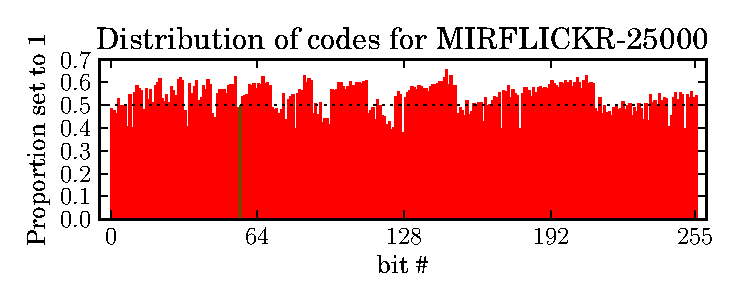
\includegraphics{test5/mirflickr.pdf}
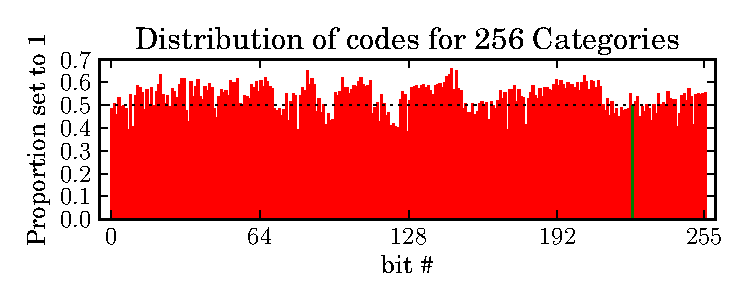
\includegraphics{test5/catagories.pdf}
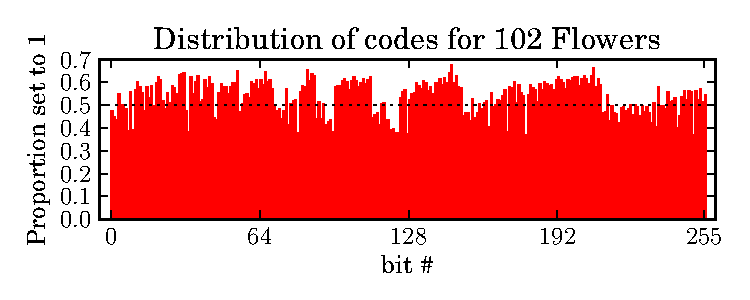
\includegraphics{test5/102flowers.pdf}
\captionsetup{width=10cm}
\caption{Empirical expected value for each bit for all codes in each of the three vision corpora used.}
\label{fig:bitdist}
\end{figure}

Text below distribution

\section{Hamming Radii needed for k-NN}

We can see from the Hamming radii required for $k=10$ and $k=1000$ nearest neighbours for our three datasets that the requred radii are much larger in our 256 bit codes compared to the 64 and 128 bit codes in Figure \ref{fig:radii}. The deviation of the required radii are also much higher for our natively generated 256 bit codes.

\begin{figure}[H]
\figfont
 
\centering
\plottestIV{test4/k10_mirflickr.radii}{MIRFLICKR-25000}{10}
\plottestIV{test4/k10_catagories.radii}{256 Categories}{10}
\plottestIV{test4/k10_102flowers.radii}{102 Flower Categories}{10}
\plottestIV{test4/k1000_mirflickr.radii}{}{1000}
\plottestIV{test4/k1000_catagories.radii}{}{1000}
\plottestIV{test4/k1000_102flowers.radii}{}{1000}
\caption{Shown are the histograms of the search radii that are required to find 10-NN and 1000-NN for 256 bit codes generated using ORB from the three datasets used.}
\label{fig:radii256}
\end{figure}

\begin{figure}[H]
\centering
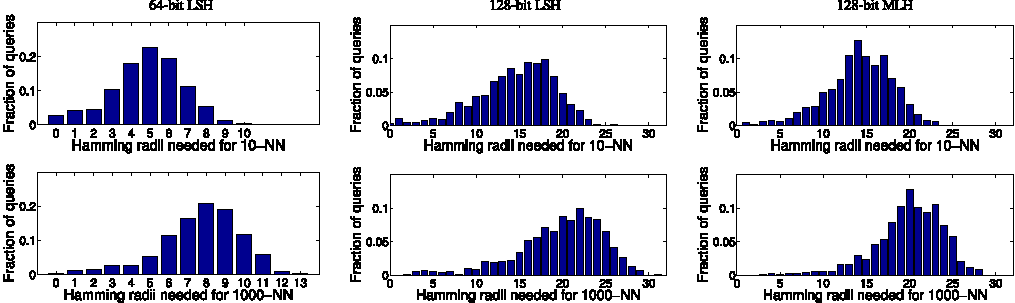
\includegraphics[width=1\textwidth]{radii64-128.pdf} 
\caption{From Norouzi \emph{et al.}~\cite{norouzi2012fast}: Shown are histograms  of the search radii that are required to find 10-NN and 1000-NN, for 64 and 128-bit code from LSH~\cite{andoni2006near}, and 128-bit codes from MLH~\cite{norouzi2011minimal}, based on 1B SIFT descriptors ~\cite{jegou2011searching}. Clearly shown are the relatively large search radii required for both the 10-NN and the 1000-NN tasks, as well as the increase in the radii required when using 128 bits versus 64 bits.
}
\label{fig:radii}
\end{figure}


\begin{figure}[p]
\figfont
\centering
\captionsetup{width=10cm}
\caption{From Norouzi \emph{et al.}~\cite{norouzi2012fast}: Recall rates for BIGANN dataset ~\cite{jegou2011searching} (1M and 1B sub-sets) obtained by K-NN on 64- and 128-bit MLH and LSH codes.}
\label{fig:hashmatching}
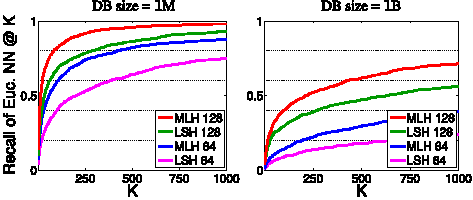
\includegraphics[width=0.5\textwidth]{LSH-MLH.pdf}
\end{figure}
\chapter{Discussion}
While the results from our testing were encouraging as to the viability of using natively generated 256 bit binary codes in a MIH structure, some discussion is warranted to explore the patterns and anomalies in the results that may elucidate further research.
%%there are still some interesting patterns in the data that should be addressed.

\section{Query Performance}
The performance tests show that our queries were running in sub-linear time up to 1000 nearest neighbours for the larger databases. It is interesting to note that for the 102 Flowers database the queries were only faster than linear scanning before $k$ reached around 250. This seems to indicate that the margin between MIH and linear scanning in terms of the query speed will increase with the database size, which is a nice result.

Also interesting is how the optimal m values were not quite as predicted. For the MIRFLICKR-25000 dataset, $m=10$ and $m=11$ were very close in terms of performance but $m=10$ was faster and the equation given by~\cite{norouzi2012fast} predicted an $m$ value closer to 11. The 256 Object Category dataset fit nicely with the predicted $m$ value. The 102 Flowers dataset was very far from the predicted optimal $m$, but it seems so far that the smaller dataset did not perform well with MIH.

It is important to note that query times were many times lower than linear scanning for small values of $k$, which means that for applications only requiring a small number of nearest neighbours MIH could be an effective technique even for small datasets. With each image having hundreds of descriptors it may not be necessary to get a large number of nearest neighbours for each descriptor to get a statistically significant match, especially since the codes have not been through a hashing function and are true nearest neighbours.

Overall, the performance of the system was good when not querying for large numbers of nearest neighbours. This could be an effect of having small datasets as with larger datasets of shorter codes, the Hamming radii required to get $k$ nearest neighbours is lower, resulting in less lookups.

\section{Code Distribution}
The calculation of the code distribution turned up the most unexpected result in all our tests. It was hypothesized that the descriptors would have a relatively uniform distribution but this turned out to be untrue. After setting up $\chi^2$ statistical tests for the bits in each dataset we found that very few of the bits could be considered uniformly distributed. What was even more interesting than that was that the codes in each dataset appeared to follow a pattern as to the mean value of each bit. This can be seen visually in our histogram of the bits in the codes. Since our datasets are fairly different in content, this pattern suggests that it is an artifact of the ORB module. More research into the methods of ORB and more statistical analyses of the codes generated may lead to smaller and better performing binary descriptors.

As well, the calculations performed in~\cite{norouzi2012fast} relied upon the assumption that the codes that were in the database were uniformly distributed. This suggests that further analysis is required to determine the effects that different distributions of codes have on the MIH query performance as descriptors from working datasets may evidently vary significantly from uniformly distributed.

\section{Hamming Radii needed for k-NN}
The Hamming radii needed for $k$-NN for our three datasets have relatively large means and deviations compared to those of the 64 and 128 bit datasets used in~\cite{norouzi2012fast}. I believe that this manifests itself as lowered performance for larger values of $k$, as we must search more buckets for codes that fall within $k$-NN. While with uniformly distributed codes the mean radii we have to search will go up with the code length it would interesting to see how the theoretical average radii compare to the empirical radii for the different dataset sizes and descriptor extraction techniques as these could indicate why the empirical optimal number of substrings $m$ did not always match the predicted optimal $m$.
%% the general formula for the radii we will have to search is $k * \frac{l}{2\log_2 n}$ where $l$ is the length of the codes and $n$ is number of codes in the database.
\chapter{Conclusion}
We have found that it is possible to quickly, efficiently and accurately match large binary codes in large databases of codes generated through ORB to perform fast image matching. This technique improves upon using hashing techniques on real valued descriptors to generate binary codes as with larger datasets these hashing techniques lose effectiveness in mapping real codes to binary codes, while binary codes generated by ORB do not suffer this degradation. As well this technique allows matching of these long binary descriptors in sub-linear times in respect to the database size. The Multi-Index hashing technique ensures that as database sizes grow the query time for these databases will increase with the square root of the size of the databases while using ORB ensures that as the database size grows the matching effectiveness of the codes will not drastically decrease. This research shows that there is promise in using natively generated binary descriptors for matching images quickly and that with current technology this technique can compete with current effective techniques.

%% This adds a line for the Bibliography in the Table of Contents.
\addcontentsline{toc}{chapter}{Bibliography}
%% ***   Set the bibliography style.   ***
%% (change according to your preference)
\bibliographystyle{plain}
%% ***   Set the bibliography file.   ***
%% ("thesis.bib" by default; change if needed)
\bibliography{thesis}

%% ***   NOTE   ***
%% If you don't use bibliography files, comment out the previous line
%% and use \begin{thebibliography}...\end{thebibliography}.  (In that
%% case, you should probably put the bibliography in a separate file
%% and `\include' or `\input' it here).

\end{document}

%%%%%%%%%%%%%%%%%%%%%%%%%%%%%%%%%%%%%%%%%%%%%%%%%%%%%%%%%%%%%%%%%%%%%%
%%  End of UOIT-THESIS.TEX
%%%%%%%%%%%%%%%%%%%%%%%%%%%%%%%%%%%%%%%%%%%%%%%%%%%%%%%%%%%%%%%%%%%%%%
